
\documentclass[10pt]{article}
\usepackage[utf8]{inputenc}
\usepackage{graphicx}
\usepackage{amsmath, amssymb}
\usepackage{geometry}
\usepackage{caption} 
\geometry{a4paper, margin=0.5in, landscape} 

\begin{document}

\section*{Comparative EIS Kinetics Report}
\textbf{Model Structure:} \texttt{R0-p(R1-p(R2-W2,CPE2),CPE1)}

\begin{center}
    
\includegraphics[width=0.45\textwidth]{../2RC_W.png}
\end{center}

\renewcommand{\arraystretch}{1.6} 
\begin{table}[h!]
    \centering
    \footnotesize
    \begin{tabular}{|l|c|c|c|c|c|c|}
        \hline
        \textbf{Element} & \textbf{Unit} & \textbf{Bounds} & \textbf{Cauvel\_1\_MBT\_24H} & \textbf{Cauvel\_1\_MBT\_48H} & \textbf{Cauvel\_1\_MBT\_72H} & \textbf{Cauvel\_1\_MBT\_168H} \\ \hline
        $R_{0}$ & $\Omega$ & $[1.0e-03, 1.0e+03]$ & $1.00e-03 \pm 6.0e+01$ & $6.66e+01 \pm 3.4e-01$ & $6.31e+01 \pm 4.1e-01$ & $2.78e+01 \pm 3.4e+01$ \\ \hline
        $R_{1}$ & $\Omega$ & $[1.0e+00, 1.0e+08]$ & $7.30e+01 \pm 6.1e+01$ & $3.98e+05 \pm 2.1e+05$ & $5.64e+05 \pm 7.3e+04$ & $4.45e+01 \pm 3.4e+01$ \\ \hline
        $R_{2}$ & $\Omega$ & $[1.0e+00, 1.0e+08]$ & $7.26e+05 \pm 7.4e+04$ & $2.27e+05 \pm 2.4e+05$ & $1.72e+05 \pm 3.2e+03$ & $1.47e+06 \pm 6.4e+05$ \\ \hline
        $W2$ & $\Omega$ sec$^{-1}$/2 & $[1.0e-05, 1.0e+07]$ & $5.78e+04 \pm 5.2e+03$ & $6.48e+04 \pm 5.6e+03$ & $1.44e+05 \pm 7.6e+03$ & $1.16e+05 \pm 3.0e+04$ \\ \hline
        $Q_{2}$ & $\Omega$$^{-1}$ sec$^{a}$ & $[1.0e-11, 1.0e-03]$ & $7.11e-06 \pm 1.7e-07$ & $1.34e-06 \pm 1.2e-06$ & $1.05e-05 \pm 7.3e-06$ & $7.95e-06 \pm 6.2e-07$ \\ \hline
        $n_{2}$ & - & $[5.0e-01, 1.0e+00]$ & $9.01e-01 \pm 2.7e-03$ & $1.00e+00 \pm 5.5e-01$ & $6.39e-01 \pm 1.6e-01$ & $8.69e-01 \pm 7.0e-03$ \\ \hline
        $Q_{1}$ & $\Omega$$^{-1}$ sec$^{a}$ & $[1.0e-11, 1.0e-03]$ & $6.35e-07 \pm 2.0e-07$ & $7.75e-06 \pm 1.2e-07$ & $8.42e-06 \pm 8.4e-08$ & $2.15e-06 \pm 4.9e-07$ \\ \hline
        $n_{1}$ & - & $[5.0e-01, 1.0e+00]$ & $5.52e-01 \pm 1.2e-01$ & $8.85e-01 \pm 2.5e-03$ & $8.70e-01 \pm 1.9e-03$ & $5.58e-01 \pm 1.1e-01$ \\ \hline
        \textbf{$\chi^2$} & - & -  & $3.214e-04$ & $4.798e-04$ & $7.795e-04$ & $6.152e-04$ \\ \hline

    \end{tabular}
\end{table}


\newpage
\section*{Analysis Results: 24H}
\begin{center}
    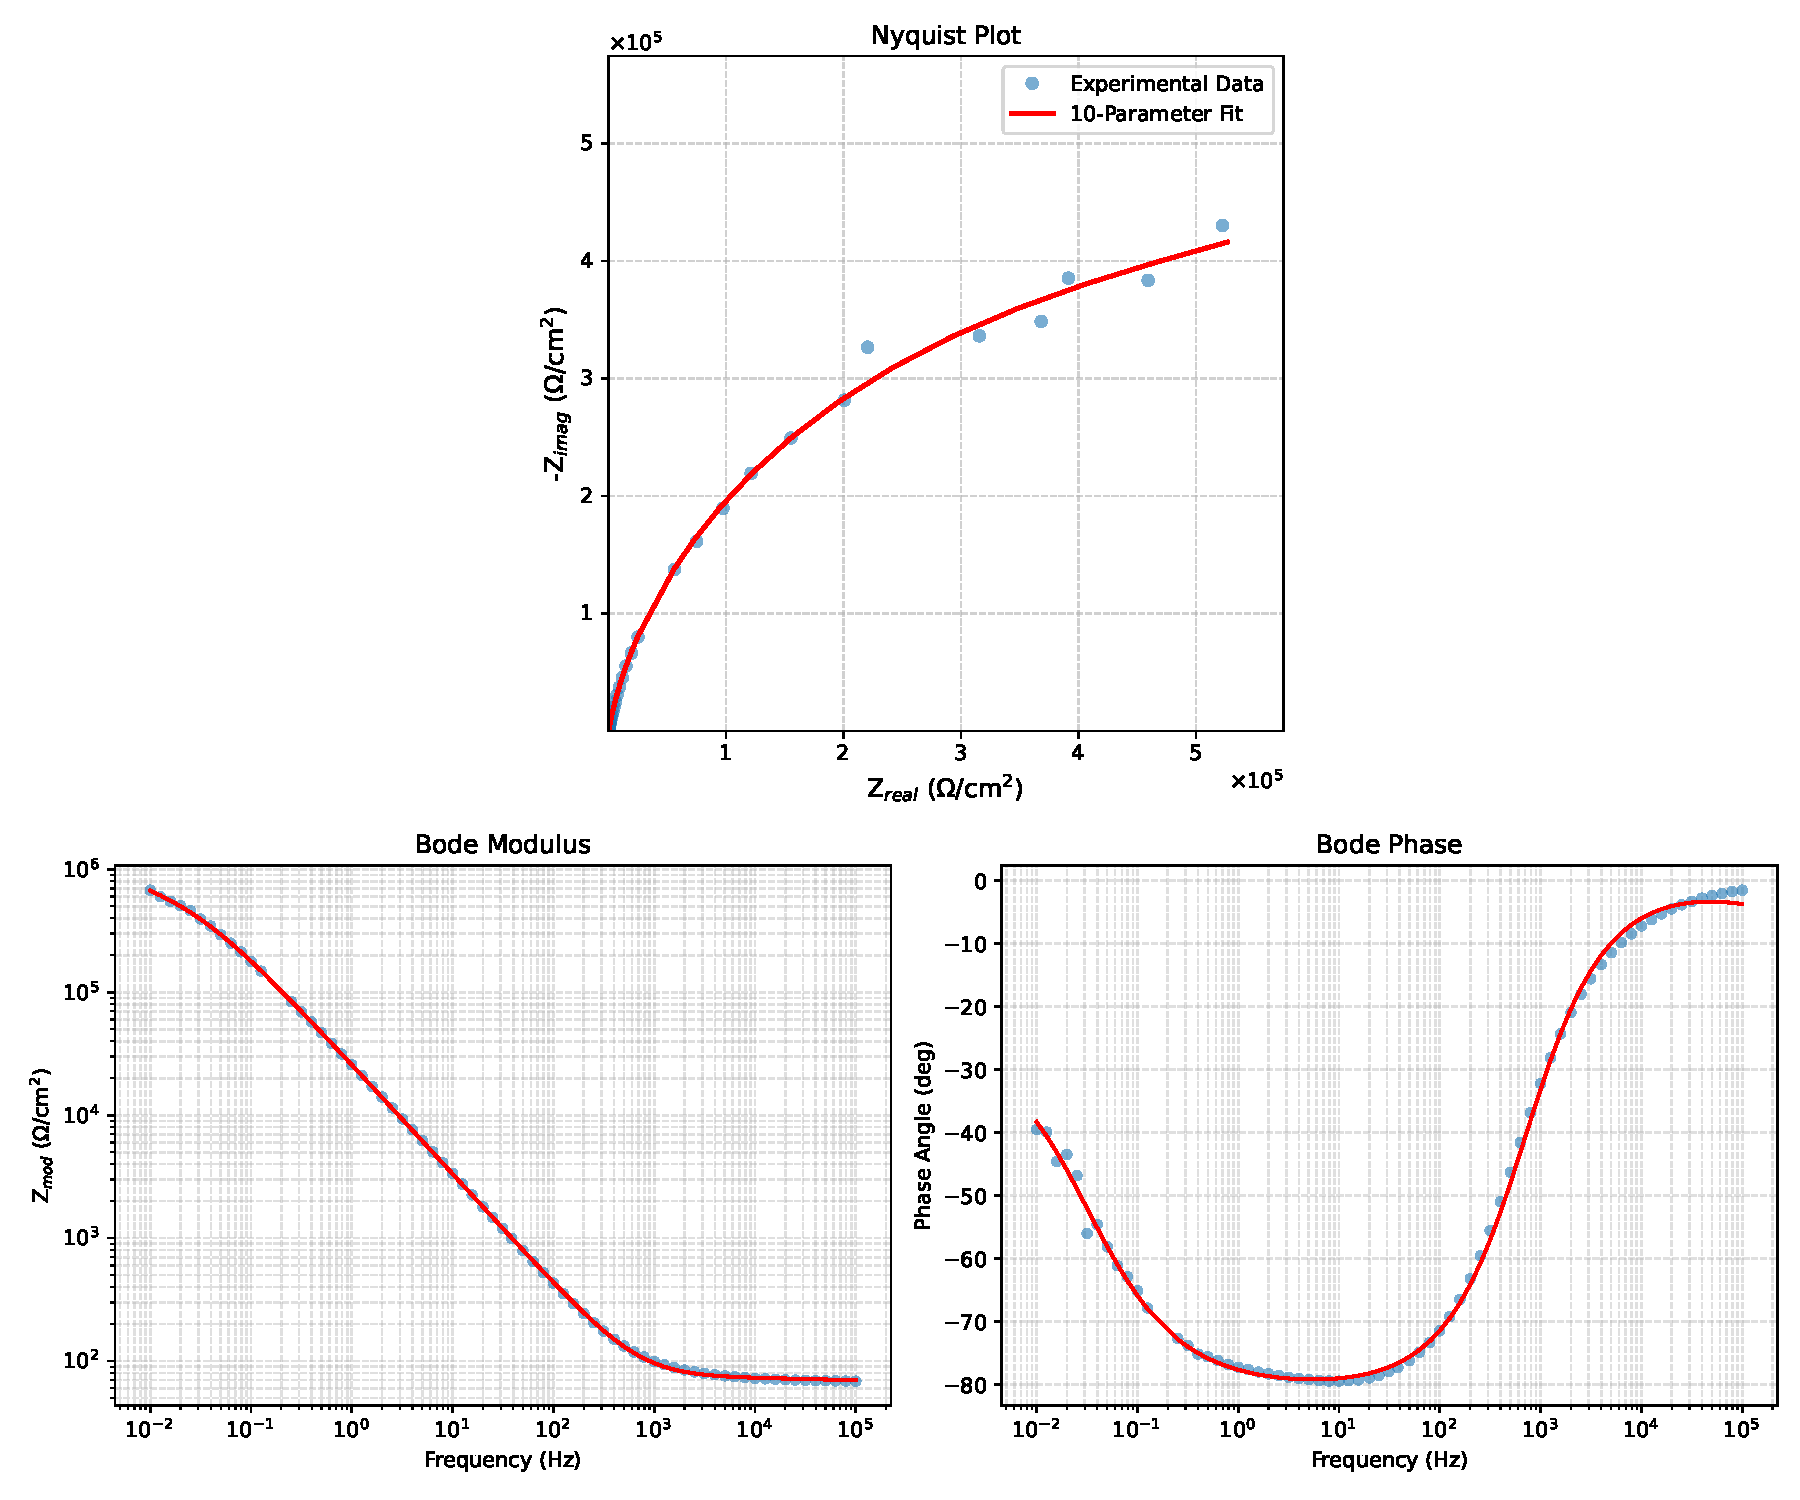
\includegraphics[width=0.7\textwidth]{plots_Cauvel_1_MBT_24H.pdf}
    \captionof{figure}{EIS Fit Results for Cauvel\_1\_MBT\_24H}
\end{center}

\newpage
\section*{Analysis Results: 48H}
\begin{center}
    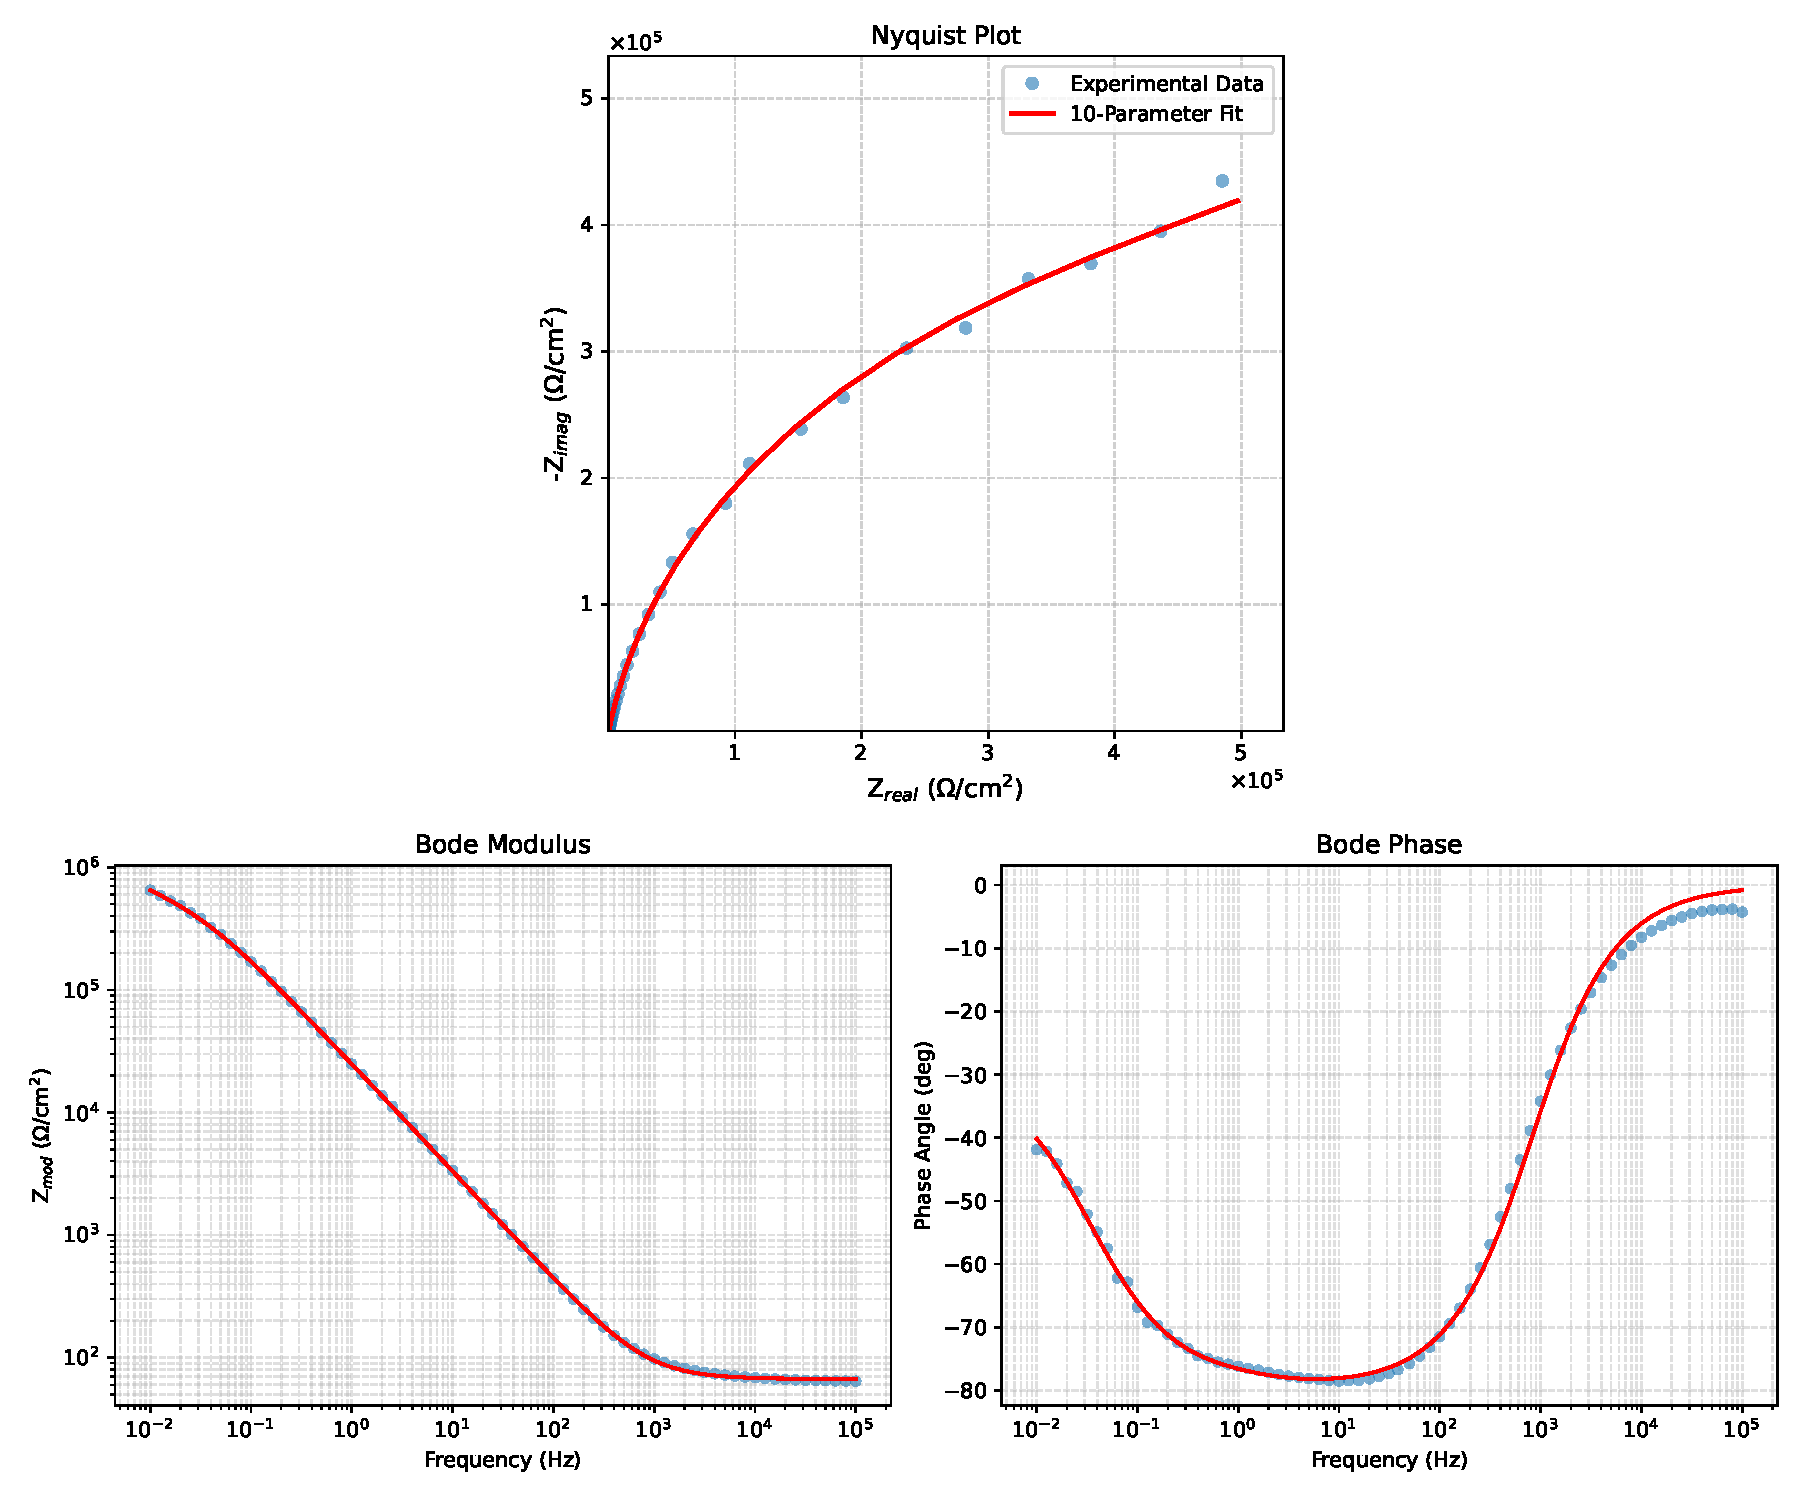
\includegraphics[width=0.7\textwidth]{plots_Cauvel_1_MBT_48H.pdf}
    \captionof{figure}{EIS Fit Results for Cauvel\_1\_MBT\_48H}
\end{center}

\newpage
\section*{Analysis Results: 72H}
\begin{center}
    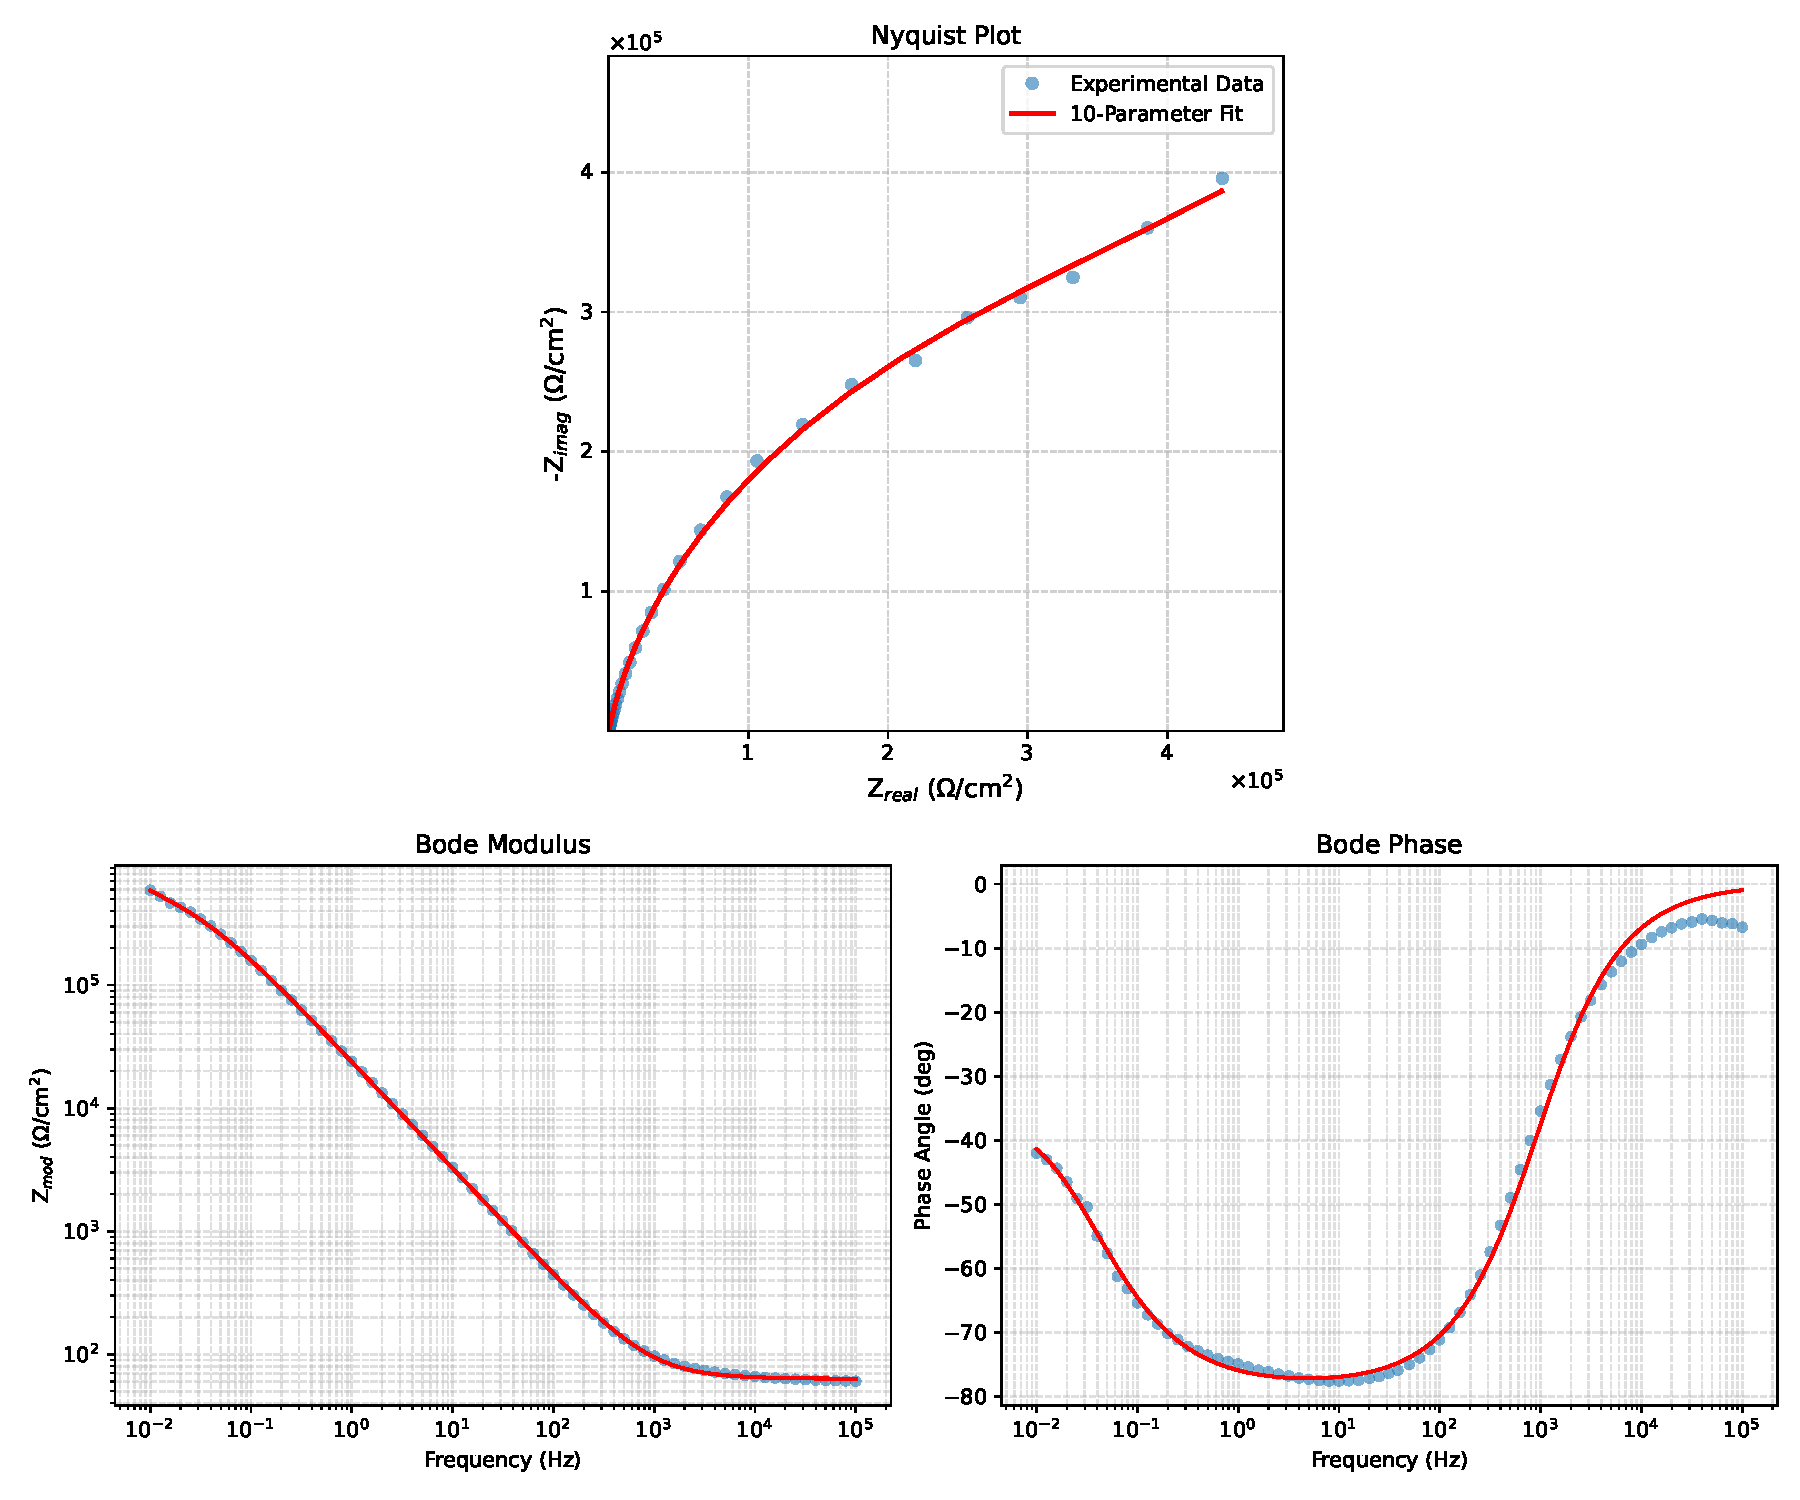
\includegraphics[width=0.7\textwidth]{plots_Cauvel_1_MBT_72H.pdf}
    \captionof{figure}{EIS Fit Results for Cauvel\_1\_MBT\_72H}
\end{center}

\newpage
\section*{Analysis Results: 168H}
\begin{center}
    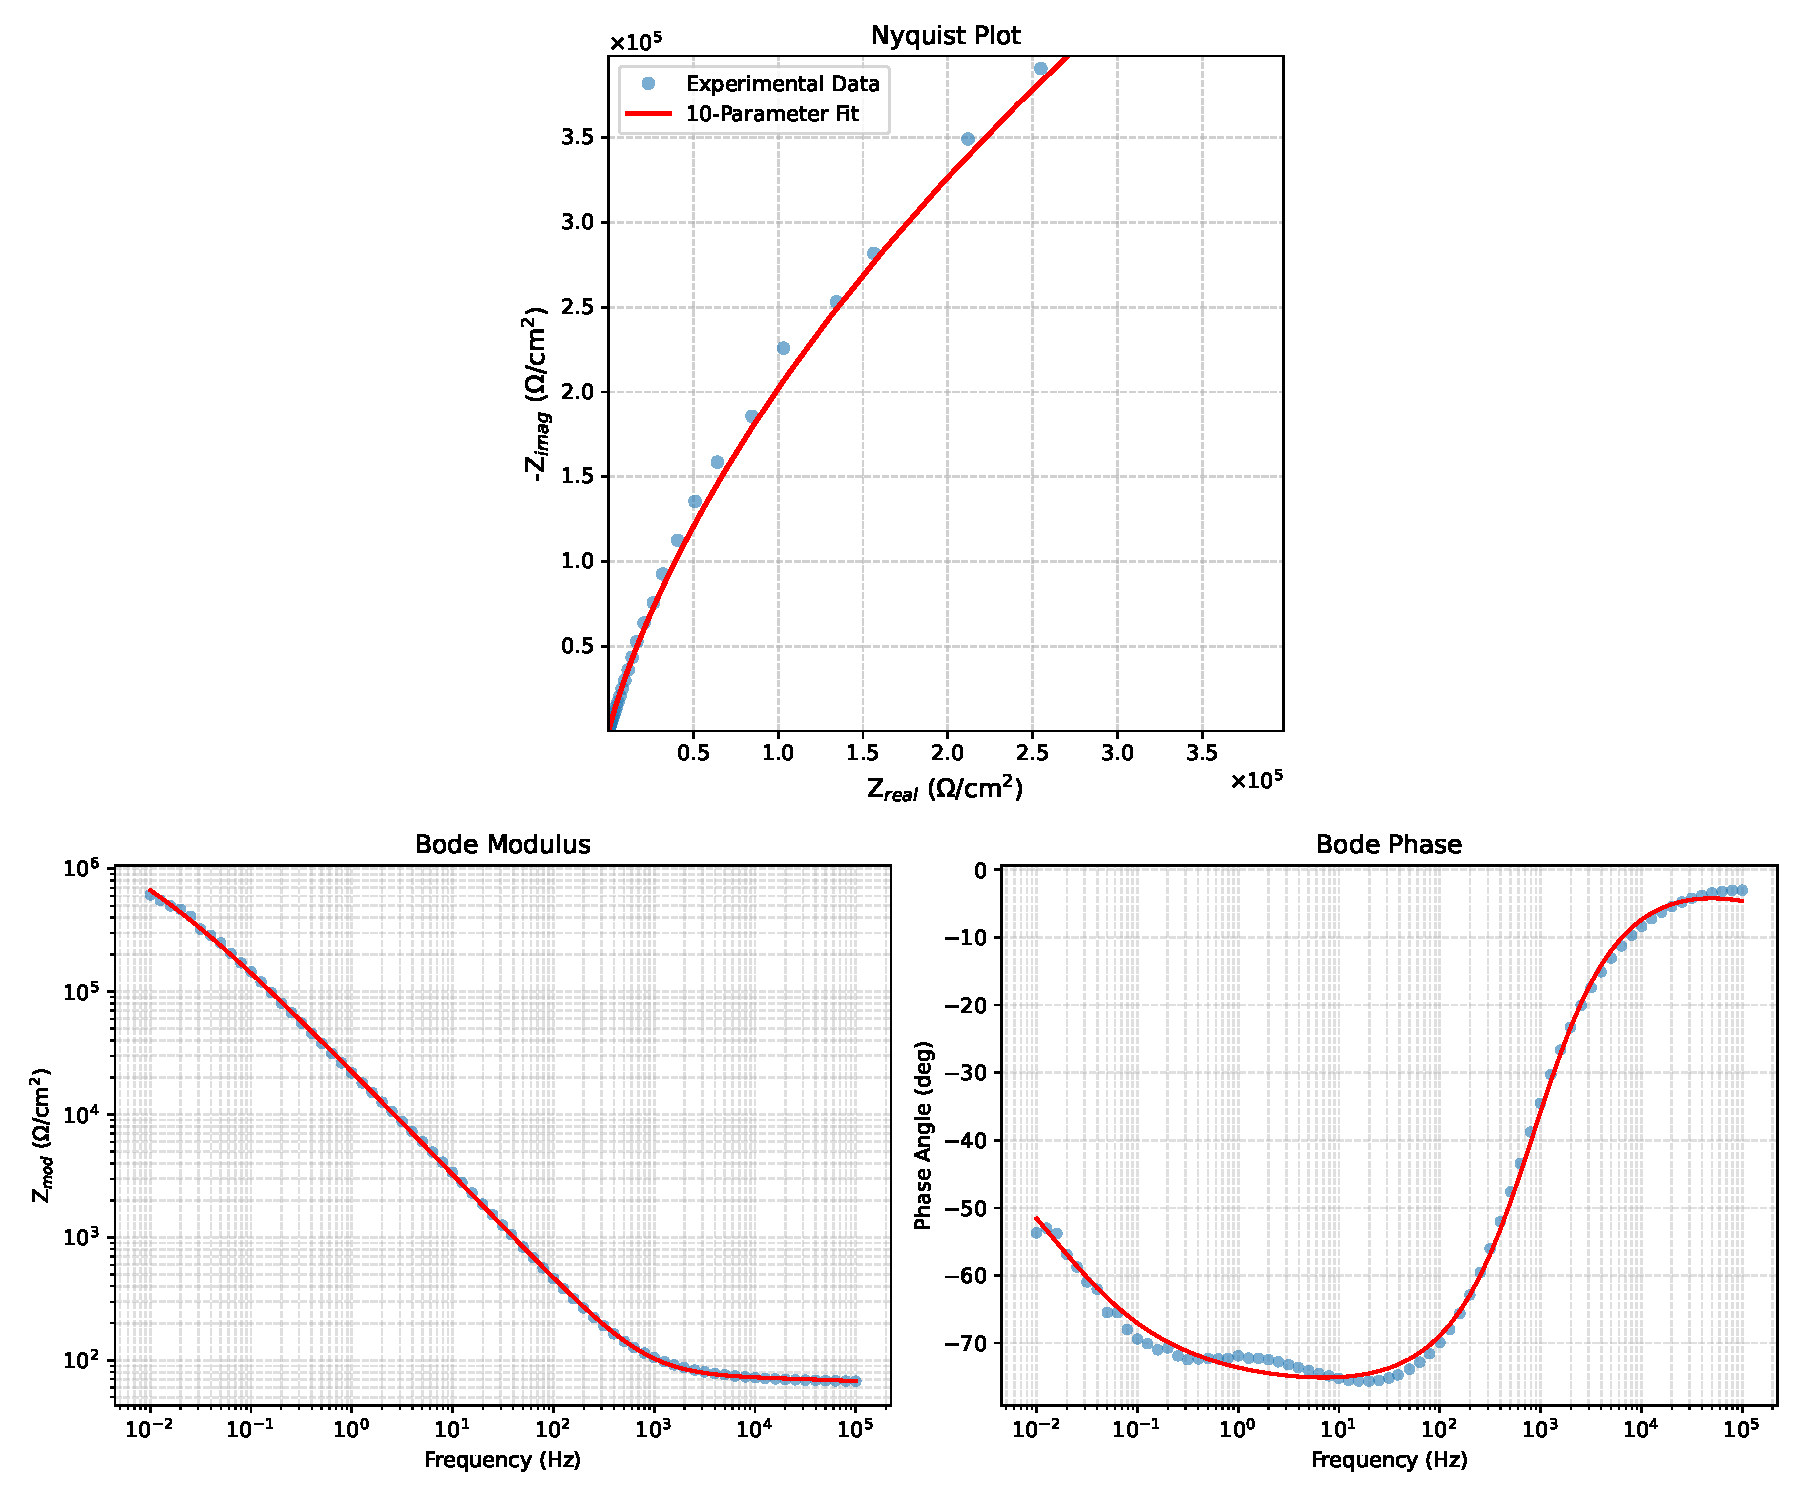
\includegraphics[width=0.7\textwidth]{plots_Cauvel_1_MBT_168H.pdf}
    \captionof{figure}{EIS Fit Results for Cauvel\_1\_MBT\_168H}
\end{center}


\end{document}
